\documentclass[letterpaper, 12pt, oneside]{tesis}

% Paquetes para idioma
\usepackage[spanish]{babel}
\usepackage[utf8]{inputenc}
\usepackage[fixlanguage]{babelbib}

% Otros paquetes instalados
% Básicos
\usepackage{natbib}
\usepackage{enumerate}

% Para dibujar figuras
\usepackage{tikz}

% Para cambiar el color de las letras
\usepackage{color}

% Para incluir código (básico)
\usepackage{verbatim}
\usepackage{fancyvrb}

% Para incluir hipervínculos
\usepackage{hyperref}
\hypersetup{urlcolor=blue, colorlinks=false}

% Para más símbolos matemáticos
\usepackage{amsmath}
\usepackage{amsthm}
\usepackage{amssymb}

% Para colocar teoremas en cajas
\usepackage{mdframed}

% Para texto Lorem Ipsum
\usepackage{blindtext}

% Para tener mas de un título
\usepackage{titling}

% Paquetes locales
% Puedes agregar paquetes locales (archivos .sty) en un subdirectorio % 'paquetes'.
% Utiliza la sintaxis \usepackage{paquetes/nombrePaquete}

% Todas las imágenes se cargan del subdirectorio 'img' por defecto.
\graphicspath{{img/}}

% Sangrías de 3 espacios (3 veces el espacio de la x)
\parindent 3ex

% Interlineado
\setlength{\baselineskip}{1.5pt}

% Interpárrafo
\setlength{\parskip}{16.5pt}

\topmargin 2cm

\renewcommand{\tablename}{Tabla}
\newcommand\listsymbolname{Acrónimos y Símbolos}

\begin{titlepage}
    \title{\vspace{-2cm} 
\includegraphics[width=1.2in]{./usb.png} \\[.2cm]
        \large Universidad Simón Bolívar \\
        Decanato de Estudios Profesionales \\
        Coordinación de Ingeniería de la Computación
        \vfill \LARGE \bfseries Desarrollo de nuevos componentes de las arquitecturas
        tecnológicas utilizadas por BBVA \vfill}
    \author{Por: \\
        Gustavo Antonio Gutiérrez Rondón \\[1.2cm]
        \bfseries{INFORME DE PASANTÍAS} \\
Presentado ante la Ilustre Universidad Simón Bolívar \\
como requisito parcial para optar al título de \\
Ingeniero de Computación}
    \date{\bfseries Sartenejas, Octubre de 2017}
\end{titlepage}

\begin{document}
\frontmatter
% Carátula
\maketitle

% Título
\begin{titlepage}
    \title{\vspace{-2cm} 
\includegraphics[width=1.2in]{./usb.png} \\[.2cm]
        \large Universidad Simón Bolívar \\
        Decanato de Estudios Profesionales \\
        Coordinación de Ingeniería de la Computación
        \vfill \LARGE \bfseries Desarrollo de nuevos componentes de las arquitecturas
        tecnológicas utilizadas por BBVA \vfill}
    \author{Por: \\
        Gustavo Antonio Gutiérrez Rondón \\[1.2cm]
        Realizado con la asesoría de: \\
        Prof. Federico Flaviani \\[1.2cm]
        \bfseries{INFORME DE PASANTÍAS} \\
Presentado ante la Ilustre Universidad Simón Bolívar \\
como requisito parcial para optar al título de \\
Ingeniero de Computación}
    \date{\bfseries Sartenejas, Octubre de 2017}
\end{titlepage}

\maketitle

\setstretch{1.3}

% Se incluye el acta de evaluación, verificar que se corresponda
% con el formato aceptado actualmente por el Decanato.
% Pagina del acta final
\begin{titlepage}
\begin{center}

% Upper part

\includegraphics[scale=0.5]{usb.png} \\

\textsc {\large UNIVERSIDAD SIMÓN BOLÍVAR} \\
\textsc{DECANATO DE ESTUDIOS PROFESIONALES\\
COORDINACIÓN DE INGENIERÍA DE LA COMPUTACIÓN}

\bigskip
\bigskip
\bigskip
\bigskip
\bigskip
\bigskip

% Title
\textsc{ACTA FINAL PROYECTO DE GRADO}

\bigskip
\bigskip

\textsc{\bfseries Desarrollo de nuevos componentes de las arquitecturas
        tecnológicas utilizadas por BBVA}
\bigskip
\bigskip
\bigskip
\bigskip

\begin{minipage}{\textwidth}
\centering
Presentado por: \\
\textsc{\bfseries Gustavo Antonio Gutiérrez Rondón} \\

\bigskip
\bigskip
\bigskip

Este Proyecto de Grado ha sido aprobado por el siguiente jurado examinador: \\

\bigskip
\bigskip

% Despues de cada line coloca el (los) nombre(s) de
% cada uno de los integrantes del jurado.
\line(1,0){200} \\
Federico Flaviani\\

\bigskip
\bigskip

\line(1,0){200} \\
@jurado1\\

\bigskip
\bigskip

\line(1,0){200} \\
@jurado2\\
\end{minipage}

\bigskip
\bigskip
\vfill

% Date/Fecha
{\large \bfseries Sartenejas, @día de @mes de 2017}

\end{center}
\end{titlepage}


% El resumen debe ser de una sola página
\addtotoc{Resumen}
\abstract{
\addtocontents{toc}{\vspace{1em}}
\blindtext

\blindtext

% Las palabras clave son generalmente los nombres de áreas de investigación a
% los cuales está asociado el trabajo. Generalmente son tres o cuatro.
\noindent \begin{small} \textbf{Palabras clave}: @palabra1, @palabra2, @palabra3.
\end{small}

% Iniciar nueva página luego del resumen
\clearpage
\setstretch{1.3}

% Begin the Dedication page

\setstretch{1.3}  % Return the line spacing back to 1.3

\pagestyle{empty}  % Page style needs to be empty for this page

\dedicatory{
    \textbf{Dedicatoria} \bigskip

    A mi familia, quienes son las bases sobre las que se levantan todos mis logros.
}

\addtocontents{toc}{\vspace{2em}}


% Agradecimientos
\acknowledgements{
\addtocontents{toc}{\vspace{1em}}
\blindtext

\blindtext
}
\clearpage

\pagestyle{fancy}

% Tabla de contenidos o índice
\lhead{\emph{Índice General}}
\tableofcontents

% Estos índices solamente se usan si el libro contiene figuras, tablas y
% algoritmos. Si alguno de estos no se utiliza, comentar o eliminar las líneas
% pertinentes.
\lhead{\emph{Índice de Figuras}}
\listoffigures

\lhead{\emph{Índice de Tablas}}
\renewcommand*\listtablename{Índice de Tablas}
\listoftables

%\lhead{\emph{Índice de Algoritmos}}
%\renewcommand*\listalgorithmname{Índice de algoritmos}
%\listofalgorithms

\setstretch{1.5}
\clearpage
\lhead{\emph{Acrónimos y símbolos}}
\listofsymbols{ll}
{

    % Aquí van las siglas
    \textbf{SIGLAS} & \textbf{S}iglas \textbf{I}sla \textbf{G}rafo
                      \textbf{L}aos \textbf{A}ve \textbf{S}erpiente\\
    \textbf{ACM} & \textbf{A}ssociation for \textbf{C}omputing \textbf{M}achinery\\
    &\\
    \hline
    &\\

    % Aquí van los símbolos
    $\iff$ & doble implicación, si y sólo si\\
    $\Rightarrow$ & implicación lógica\\
    $[u:=v]$ & sustitución textual de $u$ por $v$
}

%% ----------------------------------------------------------------
% End of the pre-able, contents and lists of things

\mainmatter
\pagestyle{fancy}

% Se incluye el cuerpo de la tesis en este documento.

\chapter*{Introducción}
\label{intro}
\lhead{\emph{Introducción}}
\addcontentsline{toc}{chapter}{Introducción}
% Organización del trabajo
% Se describe brevemente qué se hace en cada capítulo
El presente informe detalla el proceso llevado a cabo
para detectar, diseñar, implementar y probar mejoras a las arquitecturas
ePhoenix y Thin2 utilizadas en el banco español BBVA.

% Descripción del problema, de lo general hacia lo específico

El banco BBVA es una de las entidades líderes de España, con más de 10
millones de clientes y cerca de 30.000 empleados, prestando servicios
financieros a través de su red de 3200 oficinas (\cite{BBVA}). Dentro de
su área de tecnología cuenta con diferentes plataformas y arquitecturas
utilizadas con el objetivo de reducir el tiempo y homogeneizar el desarrollo.

Durante el proyecto se trabajó con dos de las arquitecturas mencionadas anteriormente.
La primera es la arquitectura ePhoenix que le permite a los equipos de desarrollo
realizar procesamientos por lotes y publicar servicios web. La segunda arquitectura
con la que se trabajó fue la arquitectura Thin2, la cual es un conjunto de librerías
basadas en Angular que le permite a los desarrolladores construir eficientemente
aplicaciones web.

\section*{Planteamiento del problema}

Con la finalidad de mantener las arquitecturas utilizadas en el banco lo
más actualizadas posibles es necesario un proceso constante de revisión y mejoras de
las mismas. Este proceso incluye una fase de levantamiento de requerimientos
para identificar fallas o posibles mejoras de las plataformas utilizadas. Luego,
una etapa de diseño de solución que solvente la deuda técnica detectada, para
finalmente pasar al desarrollo, prueba y despliegue de dicha solución.

Para contribuir con la actualización de ambas arquitecturas se debe realizar
una iteración de las etapas mencionadas sobre cada una de las plataformas para
así producir un evolutivo para ePhoenix y Thin2.

Durante el proceso de exploración se detectó que en la arquitectura ePhoenix sólo
se podían realizar conexiones a bases de datos de tipo Oracle, lo cual es una limitante
debido a que buena parte de la información manejada por el banco se encuentra en
bases de datos de otros manejadores, como PostgreSQL y Microsoft SQL Server.

Asimismo se detectó que en eld esarrollo de aplicaciones web existen operaciones
repetitivas y tediosas que enlentecen el proceso de desarrollo. Entre estas
operaciones se incluye la creación de tabla de datos, la cual involucra
un proceso bastante repetitivo.

\section*{Justificación e importancia}
Una de las constantes a la hora de desarrollar software es que los
requerimientos pueden cambiar a lo largo del tiempo. Ésto también
es cierto para los empleados encargados de desarrollar aplicaciones
dentro del banco BBVA. Debido a ésto es importante que las arquitecturas
que se utilicen para desarrollar soluciones tecnológicas, en específico
las arquitecturas ePhoenix y Thin2, se mantengan actualizadas y se mejoren
para poder satisfacer todas las necesidades de los desarrolladores.

La ventaja de mantener actualizadas las herramientas utilizadas es que le permite
a las empresas optimizar los procesos de desarrollo tecnológico que se realicen al
eliminar o mejorar los impedimentos que afectan al desarrollo de aplicaciones.

\section*{Objetivos}
A continuación se detallan el objetivo general y los objetivos específicos que
se buscan lograr en el desarrollo del proyecto.
% Objetivo general
\subsection*{Objetivo General}
El objetivo general de la pasantía es identificar posibles mejoras para las arquitecturas
de desarrollo ePhoenix y Thin2 utilizadas en el banco BBVA, y una vez
identificadas diseñar e implementar dichas mejoras para incorporarla dentro de los
estándares de arquitectura de la empresa y así enriquecer la experiencia de los
desarrolladores.
% Objetivos específicos
\subsection*{Objetivos Específicos}
\begin{itemize}
  \item Levantar información de uso de la arquitectura ePhoenix.
  \item Una vez identificada una carencia, diseñar una solución para
        mejorar la arquitectura.
  \item Implementar y probar la solución diseñada en ePhoenix.
  \item Levantar información de uso de la arquitectura Thin2.
  \item Una vez identificada una carencia, diseñar una solución para
        mejorar la arquitectura Thin2.
  \item Implementar y probar la solución diseñada en Thin2.
  \item Documentar y divulgar las mejoras implementadas para su
        posterior uso por los equipos de desarrollo del banco.
\end{itemize}

El documento se organiza en capítulos de la siguiente forma: la
Introducción al proyecto de Pasantías; en el Capítulo 1 se menciona
el contexto empresarial y el cargo ocupado en la
consultora Everis durante la pasantía; en el Capítulo 2 se explican
los fundamentos teóricos necesarios para la comprensión del problema y
la solución planteada; en el Capítulo 3 se detallan las tecnologías
implicadas en el proceso de desarrollo del proyecto; en el Capítulo 4 se
explica el funcionamiento de la metodología de gestión de proyectos utilizada
(SCRUM); en el Capítulo 5 se describen las actividades realizadas;
finalmente se le dan al lector las Conclusiones y recomendaciones.


% El número de capítulos varía. En mi libro fueron cuatro (sin contar
% introducción y conclusión).
\chapter{Entorno Empresarial}
\label{capitulo1}
\lhead{Capítulo 1. \emph{Entorno Empresarial}}

% De qué va a tratar el capítulo
% El capítulo 1 suele ser el marco teórico.

\section{@sección}
\begin{definition}
\label{definicion1}
, donde:
\begin{itemize}
\item $X$ es $\gamma - 2$.
\item $A$ es un conjunto de \textbf{cosas}.
\end{itemize}
\end{definition}

La Figura \ref{usb} muestra el símbolo de nuestra universidad.
\begin{figure}[h!]
\centering

\includegraphics[width=0.4\textwidth]{usb.png}
\caption[La popular \textit{cebolla}]{La popular \textit{cebolla}, símbolo de la USB.}
\label{usb}
\end{figure}

\begin{verbatim}
para escribir código
    básico
\end{verbatim}

\begin{Verbatim}[commandchars=\\\{\}, codes={\catcode`$=3\catcode`^=7}]
var x = 21;
if (esto_es_código) {
    imprimir(foo);
}
(lisp (listas (?paréntesis))
\end{Verbatim}

\begin{mdframed}
\begin{theorem}
\label{principal}
\textbf{Propiedades formales}
\end{theorem}
\end{mdframed}

\subsection{@subsección}
\subsubsection{@subsubsección}

La Figura \ref{grafo} lo muestra.

\shorthandoff{<>."}
\begin{figure}[h]
\begin{center}
\begin{tikzpicture}[shorten >=1pt, thick]%[shorten >=1pt,node distance=2cm,>=stealth',thick]
  \node [shape=circle,fill=black,inner sep=1.5pt,label=below:$s$] (q0) at (0,0) {};
  \node [shape=circle,fill=black,inner sep=1.5pt,label=below:$1$] (q1) at (2,0) {};
  \node [shape=circle,fill=black,inner sep=1.5pt,label=below:$t$] (q2) at (4,0) {};
  \path[->] (q0) edge (q1) (q1) edge (q2);
\end{tikzpicture}
\end{center}
\caption[@descripcionCorta]{@descripcionLarga}
\label{grafo}
\end{figure}

\begin{enumerate}[--]
\item 1
\item 2
\item 3
\end{enumerate}

\begin{tabular}{ll}
1 & 2\\ \hline
1 & 2\\
1 & 2\\
\end{tabular}

Tabla \ref{tabla:resultados}.

\begin{figure}[h]
\begin{alignat*}{1}
A\   & \longrightarrow B \mid C\\
\end{alignat*}
\caption[Gramática]{Gramática de un lenguaje.}
\label{gram}
\end{figure}

\begin{table}[h!]
\begin{center}
\begin{tabular}{llllll}
\multicolumn{4}{@{}c}{Nombre del experimento} \\
\midrule
              &    éxitos/intentos & tiempo (ms) & espacio (kB) \\
\midrule
instancia1          &        28/30 &    23 &       1.7 \\
instancia2          &        50/70 &    12 &       32.7 \\
\midrule
\end{tabular}
\end{center}
\caption[Resultados X/Y]{Resultados de X para Y}
\label{tabla:resultados}
\end{table}

\begin{equation}
\label{eq}
\Phi = (\forall x) (R x)
\end{equation}

En el Apéndice \ref{apendiceA} se encuentra.

\chapter{Marco Teórico}
\label{capitulo2}
\lhead{Capítulo 2. \emph{Marco Teórico}}

A continuación se detallan los aspectos teóricos sobre los cuales se basan
tanto las herramientas utilizadas en la pasantía como la solución propuesta
en este proyecto:

\section{API}
Un API (\emph{Application Programming Interface}) es un conjunto de comandos,
funciones, protocolos o métodos que le permiten a un programa comunicarse
con un sistema externo o librería. Las APIs permiten que varios sistemas
informáticos (Sistemas Operativos, aplicaciones, etc.) se comuniquen sin la
necesidad de exponer la funcionalidad interna de cada sistema. A su vez esto
le permite a los desarrolladores utilizar funcionalidades de otras aplicaciones
sin la necesidad de reescribir código (\cite{API}).

\section{Bases de datos relacional}

Una base de datos es un medio para almacenar y recuperar información. En términos simples
una base de datos relacional es aquella en la que la información es almacenada en tablas con
filas y columnas. Se le hace referencia a las tablas como relaciones ya que representa una
coleccion de objetos del mismo tipo. La habilidad de recuperar información relacionada de una
tabla es la base para el término Base de datos relacional (\cite{RELACIONAL}).

\section{Desarrollo Orientado a Componentes}

Este método de diseño de software establece que a la hora de construir un sistema
informático, las funcionalidades de éste sean separadas en unidades más pequeñas
llamadas componentes. Un componente es una pieza de software que ofrece a través
de una interfaz un servicio predefinido y que es capaz de comunicarse con otros
componentes (\cite{COMPONENT}). Esta estrategia de desarrollo trae como resultado
software que puede ser reutilizado con mayor facilidad y que es fácilmente escalable
agregando futuros componentes que agreguen nuevas funcionalidades. Además, facilita la
mantenibilidad del código, debido a que la encapsulación de las funcionalidades permite
detectar con mayor facilidad de donde proviene una falla.

\section{Modelo Vista Controlador}
Modelo-Vista-Controlador (MVC) es un patrón de diseño de software, especialmente útil
para diseñar interfaces de usuario. Se basa en la separación de los datos y lógica de
negocio, la interfaz gráfica a mostrar y el módulo encargado de atender y responder a
los eventos generados por el usuario en tres componentes distintos (\cite{MVC}). Estos
componentes quedan definidos de la siguiente manera:

\begin{itemize}
  \item \textbf{Modelo}: se encarga de representar los datos que maneja el sistema y
  la funcionalidad asociada que tengan estos modelos.
  \item \textbf{Vista}: está a cargo de mostrar la representación visual del modelo
  para que el usuario interactúe fácilmente con el sistema.
  \item \textbf{Controlador}: es el módulo encargado de coordinar las vistas con el modelo.
  Para ello atiende los eventos que pueda generar el usuario para luego actualizar
  adecuadamente la vista y el modelo.
\end{itemize}

Este patrón de arquitectura de software se ha vuelto bastante común en el desarrollo
de interfaces de usuario por su ventajas en cuanto a reutilización y mantenibilidad
del código.

\chapter{Marco Tecnológico}
\label{capitulo3}
\lhead{Capítulo 3. \emph{Marco Tecnológico}}

En este capítulo se mencionan las herramientas utilizadas para el desarrollo
del proyecto de pasantía. Dichas herramientas son descritas brevemente y se menciona
su uso dentro de la solución planteada.

\section{Java}

Java es un lenguaje de programación de propósito general, concurrente, basado en clases
y orientado a objetos. Está diseñado para ser lo suficientemente sencillo para
que muchos programadores puedan alcanzar fluidez en el lenguaje. (\cite{JAVA})

\section{OSGI}

OSGI (\emph{(Open Service Gateway Initiative)}) es un conjunto de especificaciones
que definen un sistema dinámico formado por componentes
para Java. Estas especificaciones permiten un modelo de desarrollo donde las aplicaciones
son dinámicamente compuestas por muchos componentes reutilizables (\cite{OSGI}).

En la figura \ref{layers} se describe el modelo por capas definido por OSGI:

\begin{figure}[h!]
\centering
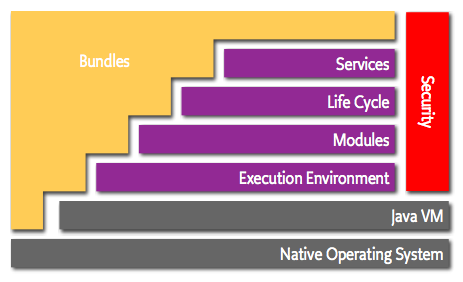
\includegraphics[width=0.4\textwidth]{layering-osgi}
\caption[Capas de OSGI]{Modelo por capas definido en OSGI. (\cite{OSGI})}
\label{layers}
\end{figure}

La siguiente lista contiene una breve descripción de los términos:
\begin{itemize}
\item \textbf{Bundles}: los Bundles son los componentes de OSGI hechos por los desarrolladores.
\item \textbf{Servicios}: la capa de servicios conecta bundles de una manera dinámica intercambiando objectos Java.
\item \textbf{Ciclo de vida}: el API para instalar, arrancar, detener, actualizar y desinstalar un bundle.
\item \textbf{Módulos}: la capa que define como un bundle puede importar y exportar código.
\item \textbf{Seguridad}: la capa que determina los aspectos de seguridad.
\item \textbf{Ambiente de Ejecución}: define que métodos y clases están disponibles en una plataforma específica.
\end{itemize}


\section{Apache Felix}

Apache Felix es un esfuerzo de la comunidad Apache para implementar la especificación de
la plataforma OSGI bajo la licencia Apache. La especificación OSGI es ideal para
cualquier proyecto interesado en los principios de modularidad, desarrollo orientado
a componentes y desarrollo orientado a servicios (\cite{FELIX}).

\section{JDBC}

El \emph{API} JDBC (\emph{Java Database Connectivity}) es el estándar en la industria
para conectividad independiente del manejador de base de datos entre programas escritos en
Java y una gran variedad de bases de datos (\cite{JDBC}). Para cada uno de los manejadores
de base de datos que se desean conectar a través de un programa Java deberá existir una implementación
del estándar JDBC, también llamado Driver, que le permite al programa comunicarse a través del
API con el manejador de base de datos.

\section{Base de datos Oracle}

La base de datos Oracle es un sistema de manejo de base de datos relacional (\cite{ORACLE})
producido y mantenido por Oracle Corporation.

\section{PostgreSQL}

PostgreSQL es un poderoso sistema de bases de datos relacional. Tiene más de
15 años de desarrollo activo y una arquitectura que se ha ganado la reputación de tener
integridad de datos, confiabilidad y correctitud de datos (\cite{POSTGRE}).

\section{Microsoft SQL Server}
Microsoft SQL Server es un sistema de manejo de bases de datos relacional desarrollado por
Microsoft.

\section{Arquitectura ePhoenix}

Construido sobre la base de Apache Felix, la arquitectura ePhoenix le brinda a los
equipos de desarrollo del BBVA todas las herramientas necesarias para desarrollar programas
que realicen procesamiento por lotes o publiquen servicios web. Cuando un equipo de
desarrolladores se disponga a realizar aplicaciones con esta arquitectura se le despliegan
en un servidor dedicado Apache Félix junto con los bundles que conforman ePhoenix para
que los desarrolladores desplieguen sus propios bundles que implementen su lógica de negocio.

Abarcar todas las funcionalidades que ofrece la arquitectura escapa del alcance del
proyecto de pasantías, por lo que se trabajará con los componentes de ePhoenix
que se encargan de realizar las conexiones a bases de datos usando JDBC.

\section{HTML}

HTML, que significa Lenguaje de Marcado para Hipertextos (HyperText Markup Language)
es el elemento de construcción más básico de una página web y se usa para crear y
representar visualmente una página web. Determina el contenido de la página web,
pero no su funcionalidad (\cite{HTML}).

\section{Javascript}

JavaScript es un lenguaje ligero e interpretado, orientado a objetos, más conocido
como el lenguaje de script para páginas web. Es un lenguaje script multi-paradigma, dinámico,
soporta estilos de programación funcional, orientada a objetos e imperativa (\cite{JS}).

\section{Node.js}
Node.js es un entorno de ejecución para JavaScript construido con el motor de JavaScript V8
de Chrome. Node.js usa un modelo de operaciones de entrada y salida sin bloqueo y orientado a eventos.
El ecosistema de paquetes de Node.js, npm, es el ecosistema mas grande de librerías
de código abierto en el mundo (\cite{NODE}).

\section{JSON}
JSON (\emph{JavaScript Object Notation}) es un formato de intercambio de datos ligero.
Esta diseñado para ser fácil de leer y escribir por humanos y fácil de parsear y generar
por las máquinas (\cite{JSON}).

\section{Angular}
Angular es una plataforma escrita en JavaScript que facilita el proceso
de crear aplicaciones para la web. Angular combina plantillas declarativas, inyección de dependencias
y buenas prácticas integradas para solucionar problemas a la hora de desarrollar (\cite{ANGULAR}).
Además, al presentar una arquitectura que combina el desarrollo orientado a componentes
y el patrón de diseño MVC, Angular ofrece grandes ventajas en cuanto a mantenibilidad
y reusabilidad de código.

\section{Arquitectura Thin2}

A diferencia de ePhoenix, Thin2 no está basado en OSGI.
Para Thin2 se tomó como base el framework de aplicaciones web Angular. Partiendo
de la capacidad de Angular de definir componentes reutilizables se le ofrecen a los
equipos de desarrollo varios elementos predefinidos para realizar las tareas más
comunes a la hora de escribir una página web. Entre estos componentes se pueden
mencionar el componente para obtener configuraciones de un servidor o el que implementa
la autenticación y autorización propia manejada dentro de BBVA.

En la práctica, la arquitectura Thin2 está conformada por un conjunto de librerías
escritas con Angular puestas a la disposición de los equipos de desarrollo a través
del repositorio interno de BBVA. Una vez descargadas estas librerías junto con
Angular, los desarrolladores pueden utilizar los componentes predefinidos en la
arquitectura para realizar sus aplicaciones web.

\section{Herramientas para la gestión del proyecto}

Aparte de las tecnologías utilizadas para desarrollar el proyecto se utilizaron
las siguientes herramientas para la gestión de la pasantía y el control de versiones:

\subsection{Dimensions CM}

Dimensions CM is un gestor de cambios y configuraciones que disminuye eficientemente
la complejidad del desarrollo paralelo, integrando y automatizando prácticas de desarrollo
(\cite{DIMENSIONS}).

Dimensions CM es la herramienta utilizada en el BBVA para el control de versiones, control de
calidad y el despliegue de aplicaciones.

\subsection{Jira}

Jira Software es una herramienta de gestión de proyectos para equipos ágiles (\cite{JIRA}).
Entre sus características ofrece una manera sencilla de manejar y visualizar
las tareas asignadas mediante la metodología de trabajo SCRUM.

\chapter{@nombreCapítulo}
\label{capitulo4}
\lhead{Capítulo 4. \emph{@nombreCapítulo}}

\Blindtext


\chapter{Conclusiones y Recomendaciones}
\label{conclusiones}
\lhead{\emph{Conclusiones y Recomendaciones}}

% Incluir recomendaciones para trabajos futuros


% El estilo de la bibliografía es AAAI, definido en el archivo aaai.bst.
\label{Bibliography}
\bibliography{bibliografia}
\lhead{\emph{Bibliografía}}
\bibliographystyle{aaai}
\addtocontents{toc}{\vspace{2em}}

% Apéndices
\appendix
\chapter{Cambios en la interfaz administrativa de ePhoenix}
\label{apendiceA}
\lhead{Apéndice A. \emph{Cambios en la interfaz administrativa de ePhoenix}}

% En los apéndices se incluye cualquier información que no sea esencial para la
% comprensión básica del trabajo, pero provea ejemplos y casos de estudio
% extendidos que permitan un análisis más exhaustivo.

\begin{figure}[h!]
\centering
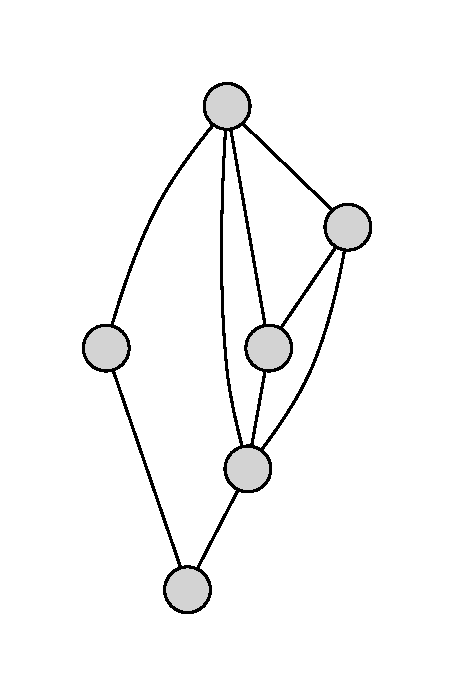
\includegraphics[width=0.5\textwidth]{grafo}
\caption[Grafo]{Grafo gris.}
\label{imagen:grafo}
\end{figure}

\begin{figure}[h!]
\centering
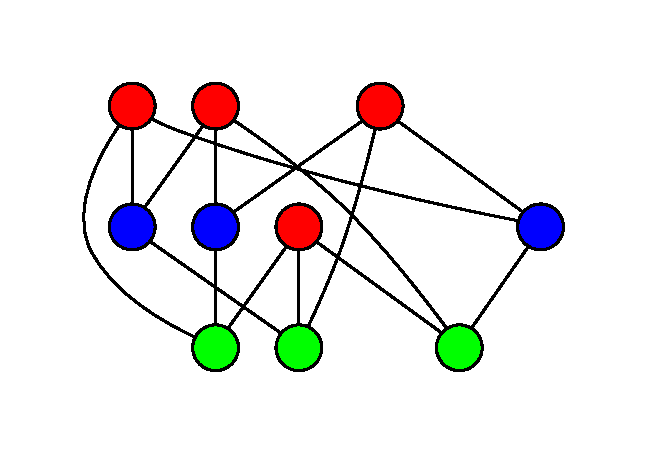
\includegraphics[width=\textwidth]{grafocolor}
\caption[Grafo coloreado (esto sale en la tabla de contenidos)]{Grafo con color.}
\label{imagen:grafodecolores}
\end{figure}

\chapter{Pantallazos de la aplicación de ejemplo para Thin2}
\label{apendiceB}
\lhead{Apéndice B. \emph{Pantallazos de la aplicación de ejemplo para Thin2}}

\begin{figure}[h!]
\centering
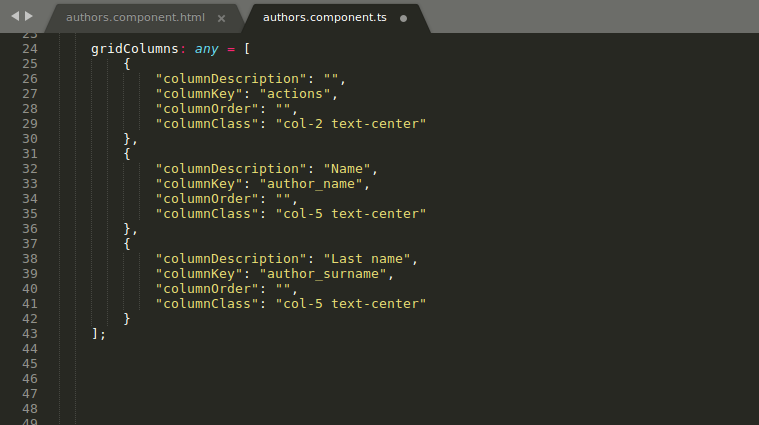
\includegraphics[width=\textwidth]{author-config}
\caption[Configuración de tabla sencilla]{Configuración de una tabla sin función.}
\label{author:1}
\end{figure}

\begin{figure}[h!]
\centering
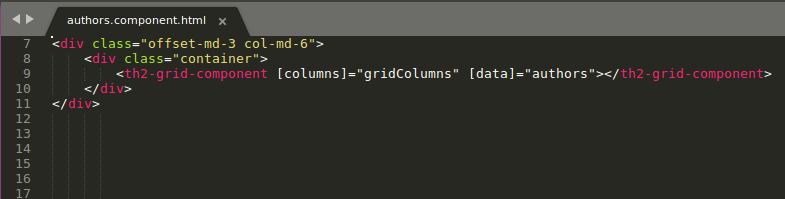
\includegraphics[width=\textwidth]{author-html}
\caption[Código html de tabla sencilla]{Código html utilizado para crear una tabla sin función.}
\label{author:2}
\end{figure}

\begin{figure}[h!]
\centering
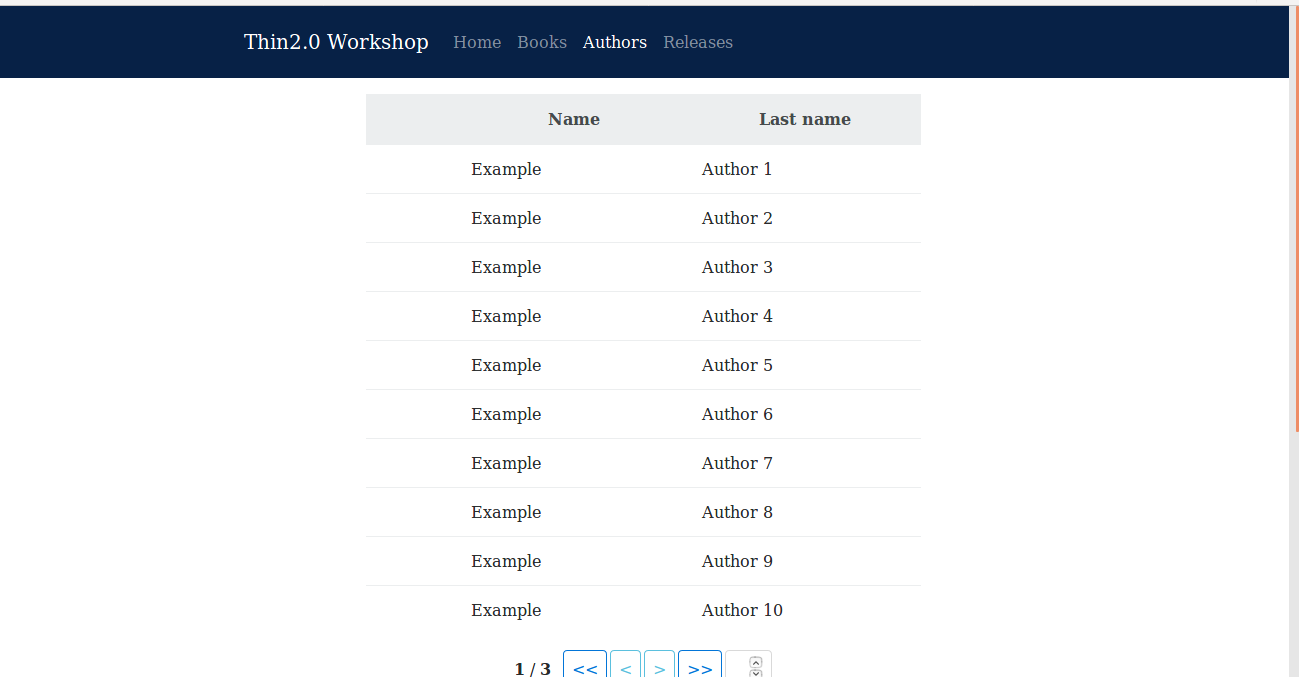
\includegraphics[width=\textwidth]{author-resultados}
\caption[Tabla sencilla en aplicación]{Resultado de la tabla realizada en la aplicación.}
\label{author:3}
\end{figure}

\begin{figure}[h!]
\centering
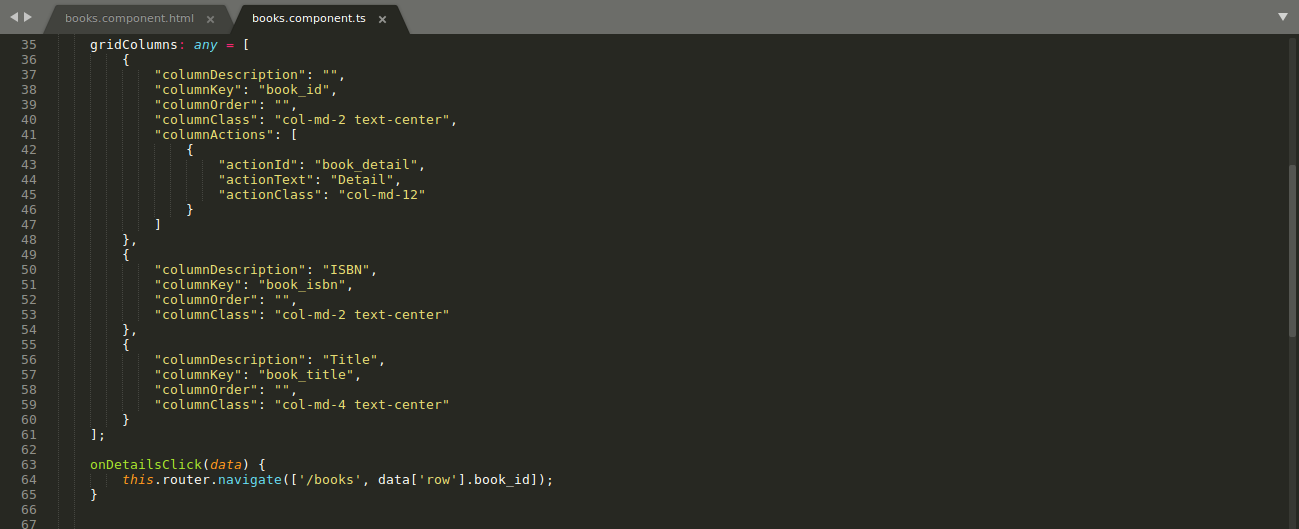
\includegraphics[width=\textwidth]{books-config}
\caption[Configuración de tabla con evento]{Configuración de una tabla con una función asociada.}
\label{books:1}
\end{figure}

\begin{figure}[h!]
\centering
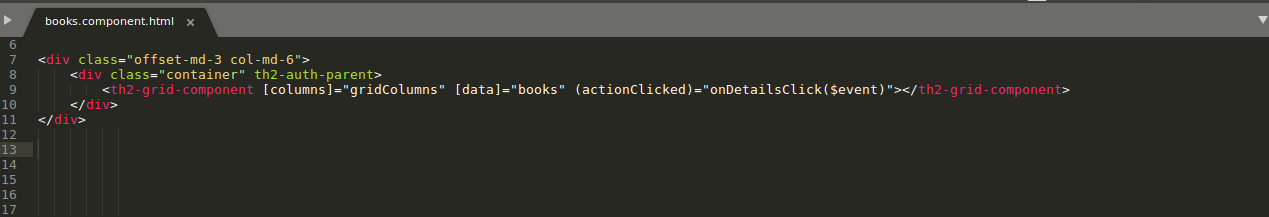
\includegraphics[width=\textwidth]{books-html}
\caption[Código html de tabla con evento]{Código html utilizado para crear una tabla con una función asociada.}
\label{books:2}
\end{figure}

\begin{figure}[h!]
\centering
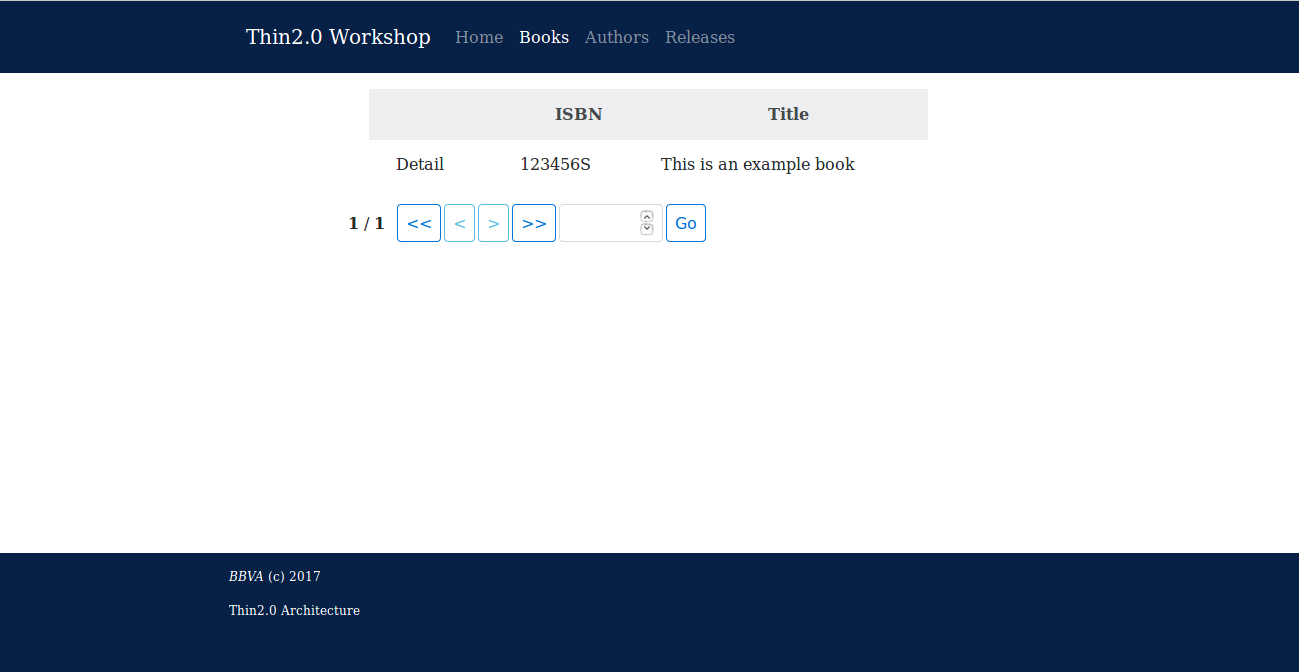
\includegraphics[width=\textwidth]{books-result}
\caption[Tabla con evento en aplicación]{Tabla con función asociada resultante en la aplicación.}
\label{books:3}
\end{figure}

\begin{figure}[h!]
\centering
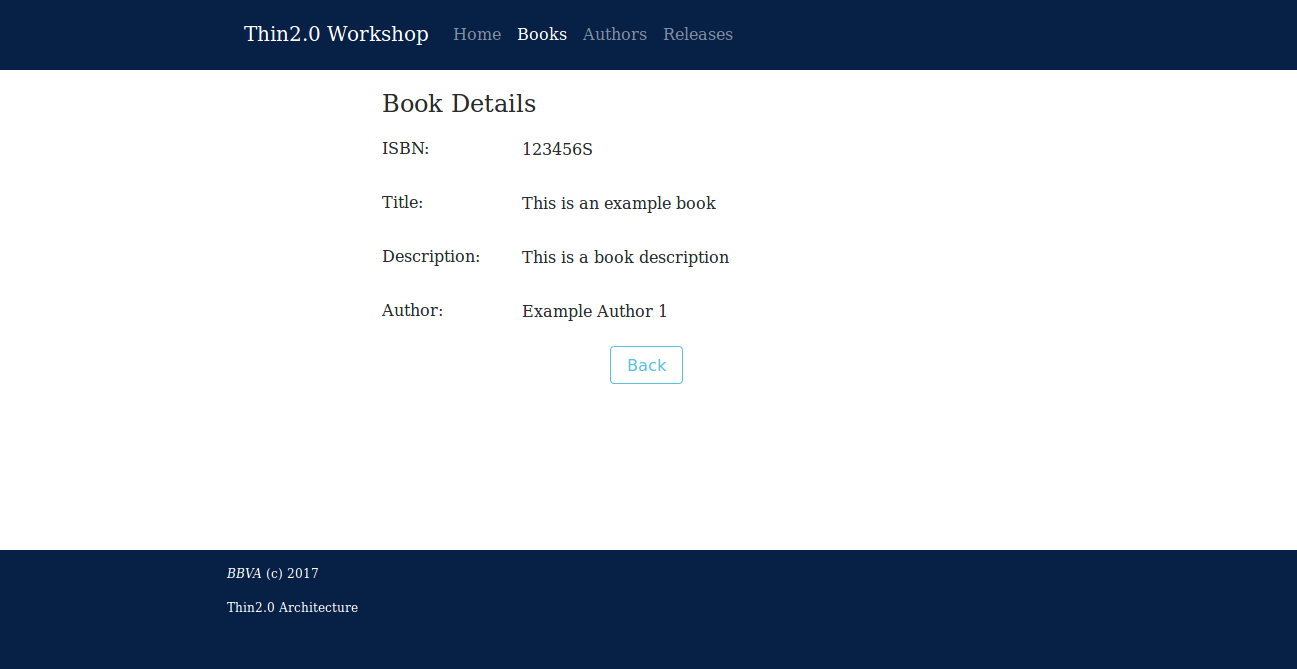
\includegraphics[width=\textwidth]{book-detail}
\caption[Página al hacer click en la tabla]{Cambio en la aplicación al ejecutar la función asociada a la celda.}
\label{books:4}
\end{figure}

\addtocontents{toc}{\vspace{2em}}

\backmatter

\end{document}
